\documentclass[onecolumn,10pt]{jhwhw}

\usepackage{epsfig} %% for loading postscript figures
\usepackage{amsmath}
\usepackage{graphicx}
\usepackage{grffile}
\usepackage{pdfpages}
\usepackage{algpseudocode}
\usepackage{wrapfig}
\usepackage{pgfplots}
\usepackage{amsfonts}
\usepackage{booktabs}
\usepackage{siunitx}
\usepackage{commath}
\usepackage{rotating}
\usepackage{url}
\usepackage{multimedia}
\usepackage{hyperref}
\usepackage{mathtools}

% Default fixed font does not support bold face
\DeclareFixedFont{\ttb}{T1}{txtt}{bx}{n}{12} % for bold
\DeclareFixedFont{\ttm}{T1}{txtt}{m}{n}{12}  % for normal

% Custom colors
\usepackage{color}
\usepackage{listings}
\usepackage{framed}
\usepackage{caption}
\usepackage{bm}
\captionsetup[lstlisting]{font={small,tt}}

\definecolor{mygreen}{rgb}{0,0.6,0}
\definecolor{mygray}{rgb}{0.5,0.5,0.5}
\definecolor{mymauve}{rgb}{0.58,0,0.82}

\lstset{ %
  backgroundcolor=\color{white},   % choose the background color; you must add \usepackage{color} or \usepackage{xcolor}
  basicstyle=\ttfamily\footnotesize, % the size of the fonts that are used for the code
  breakatwhitespace=false,         % sets if automatic breaks should only happen at whitespace
  breaklines=true,                 % sets automatic line breaking
  captionpos=b,                    % sets the caption-position to bottom
  commentstyle=\color{mygreen},    % comment style
  deletekeywords={...},            % if you want to delete keywords from the given language
  escapeinside={\%*}{*)},          % if you want to add LaTeX within your code
  extendedchars=true,              % lets you use non-ASCII characters; for 8-bits encodings only, does not work with UTF-8
  frame=single,                    % adds a frame around the code
  keepspaces=true,                 % keeps spaces in text, useful for keeping indentation of code (possibly needs columns=flexible)
  columns=flexible,
  keywordstyle=\color{blue},       % keyword style
  language=Python,                 % the language of the code
  morekeywords={*,...},            % if you want to add more keywords to the set
  numbers=left,                    % where to put the line-numbers; possible values are (none, left, right)
  numbersep=5pt,                   % how far the line-numbers are from the code
  numberstyle=\tiny\color{mygray}, % the style that is used for the line-numbers
  rulecolor=\color{black},         % if not set, the frame-color may be changed on line-breaks within not-black text (e.g. comments (green here))
  showspaces=false,                % show spaces everywhere adding particular underscores; it overrides 'showstringspaces'
  showstringspaces=false,          % underline spaces within strings only
  showtabs=false,                  % show tabs within strings adding particular underscores
  stepnumber=1,                    % the step between two line-numbers. If it's 1, each line will be numbered
  stringstyle=\color{mymauve},     % string literal style
  tabsize=4,                       % sets default tabsize to 2 spaces
}

\usepackage{etoolbox}
\renewcommand{\lstlistingname}{Diagram}% Listing -> Algorithm
\patchcmd{\thebibliography}{\chapter*}{\section*}{}{}

\author{John Karasinski}
\title{Homework 4}

\begin{document}
%\maketitle

\problem{}
\textit{Basic orbital parameters: remind yourself:}
\begin{enumerate}
\item Determine the kinetic, potential, and total energy per unit mass, and the magnitude of the moment of
momentum (or, angular momentum due to orbital motion) for the HST
\begin{align*}
p &= \dfrac{h^2}{\mu} = \dfrac{52519.6585^2}{398600.4} = 6920 km\\
r &= \dfrac{p}{1 + e \cos{\theta}} = \dfrac{6920}{1 + 0.0002935 \cos{0.5652}} = 6918.285 km\\
\\
\mbox{alt} &= \left( a (1-e \cos{E}) \right) - 6378 \mbox{ km} \\
           &= \left( 6920 (1-0.0002935 \cos{5.71815}) \right) - 6378 \\
           &= 540.28 \mbox{ km} \\
\mbox{vel} &= \sqrt{\mu \left( \dfrac{2}{\mbox{alt} + 6378} - \dfrac{1}{a} \right)} \\
           &= \sqrt{398600.4 \left( \dfrac{2}{540.28 + 6378} - \dfrac{1}{6920} \right)} \\
           &=13.1465 \mbox{ km/s}\\
\\
\epsilon_p &= - \dfrac{\mu}{r} = - \dfrac{398600.4}{6918.285} = -57.615 \dfrac{J}{kg} \\
\epsilon_k &= \dfrac{v^2}{2} = \dfrac{13.1465^2}{2} = 86.41614 \dfrac{J}{kg} \\
\epsilon &= \epsilon_k + \epsilon_p = \dfrac{v^2}{2} - \dfrac{\mu}{r} = 28.80114 \dfrac{J}{kg} \\
\\
h &= \sqrt{a(1-e^2)\mu} \\
  &= \sqrt{6920 (1-(0.0002935)^2) 398600.4} \\
  &= 52519.6585 \mbox{ km$^2$/s}
\end{align*}
\end{enumerate}

\clearpage
\problem{}
% http://www.orbiter-forum.com/showthread.php?t=26682
\textit{Assume your spacecraft is an elliptical transfer orbit, with perigee of 150km above Earth mean surface, and apogee at HST mean altitude.}

HST mean altitude is 552.7km.
\begin{enumerate}
\item Compute the value (deg) of the true anomaly one hour after perigee passage.
\begin{align*}
R_a &= 552.7 \mbox{ km} + 6378 \mbox{ km} = 6930.7 \mbox{ km}\\
R_p &= 150 \mbox{ km} + 6378 \mbox{ km} = 6528 \mbox{ km}\\
a &= \dfrac{R_a + R_p}{2} = 6729.35 \mbox{ km}\\
e &= \dfrac{R_a - R_p}{R_a + R_p} = 0.0299 \\
M_m &= \sqrt{\dfrac{\mu}{a^3}} = \sqrt{\dfrac{398600.4}{(6729.35)^3}} = 0.0011\\
% T &= 2 \pi \sqrt{\dfrac{a^3}{\mu}} = 2 \pi \sqrt{\dfrac{(6729.35)^3}{398600.4}} = 5493.7726 \mbox{ s}\\
% M &= E - e \sin{E}
M &= M_m \cdot t = 0.0011 \cdot 60 \cdot 60 = 3.96 \mbox{ rads}\\
E &= E_o - \dfrac{E_o - e \sin{E_o} - M}{1 - e \cos{E_o}} \\
  &= M - \dfrac{M - e \sin{M} - M}{1 - e \cos{M}} \\
  &= 3.96 - \dfrac{3.96 - 0.299 \sin{3.96} - 3.96}{1 - 0.299 \cos{3.96}} \\
  &= 3.7787 \mbox{ rads}\\
\nu &= \cos^{-1}\left({\dfrac{\cos{E} - e}{1 - e \cos{E}}}\right) \\
    &= \cos^{-1}\left({\dfrac{\cos{3.7787} - 0.0299}{1 - 0.0299 \cos{3.7787}}}\right) \\
    &= 2.5220
\end{align*}
\item Compute the magnitude of the Earth-relative velocity of your spacecraft at this same point
\begin{align*}
\mbox{alt} &= \left( a (1-e \cos{E}) \right) - 6378 \mbox{ km} \\
           &= \left( 6729.35 (1-0.0299 \cos{3.7787}) \right) - 6378 \\
           &= 513.0846 \mbox{ km}\\
\mbox{vel} &= \sqrt{\mu \left( \dfrac{2}{\mbox{alt} + 6378} - \dfrac{1}{a} \right)} \\
           &= \sqrt{398600.4 \left( \dfrac{2}{\mbox{513.0846} + 6378} - \dfrac{1}{6729.35} \right)} \\
           &= 7.5135 \mbox{ km/s}
\end{align*}
\end{enumerate}

\clearpage
\problem{}
\textit{Obtain the Two-Line-Element for HST at an epoch of your choosing.}
% http://www.satellite-calculations.com/TLETracker/SatTracker.htm
\begin{verbatim}
HST
1 20580U 90037B   16031.61163492  .00001273  00000-0  69179-4 0  9996
2 20580  28.4704  87.0856 0002935 165.2440 327.6400 15.08104961214326

Epoch Time: Sun Jan 31 2016 06:40:45 GMT-0800 (PST)
\end{verbatim}
\begin{enumerate}
\item Write down the 6 orbital elements h, e, I, $\Omega$, $\omega$, and $\theta$\\
I = inclination = 28.4704 deg = 0.4969 rad\\
$\Omega$ = right ascension of ascending node = 87.0856 deg = 1.5199 rad\\
e = eccentricity = 0.0002935\\
$\omega$ = argument of perigee = 165.2440 deg = 2.8841 rad\\
M = Mean Anomaly = 327.640 deg = 5.7184 rad\\
n = Mean Motion = 15.08104961 rev/day = 0.00109672488 rads/s
\begin{align*}
\theta = \mbox{true anomaly} &= \cos^{-1}\left({\dfrac{\cos{E} - e}{1 - e \cos{E}}}\right) \\
       &= \cos^{-1}\left({\dfrac{\cos{5.71815} - 0.0002935}{1 - 0.0002935 \cos{5.71815}}}\right) \\
       &= 0.5652 \mbox{ rad}\\
a &= \left(\dfrac{\mu}{n^2}\right)^{1/3} \\
  &= \left(\dfrac{398600.4}{(0.00109672488)^2}\right)^{1/3} \\
  &= 6920 \mbox{ km}\\
h = \mbox{angular momentum} &= \sqrt{a(1-e^2)\mu} \\
  &= \sqrt{6920 (1-(0.0002935)^2) 398600.4} \\
  &= 52519.6585 \mbox{ km$^2$/s}
\end{align*}

\item Also compute the eccentric anomaly E.
\begin{align*}
M &= E - e \sin{E} \\
5.7184 &= E - 0.0002935 \sin{E} \\
E &= 5.71815 \mbox{ rad, via Newton-Raphson method} \\
\end{align*}
\item Using class notes (Lecture 7, Thurs 1/26/16, ``Compute State Vector from Orbital Elements''), find the HST state vector at this time, in the geocentric equatorial reference frame. (Also see Curtis book, Sec 4.6 and App D2 (SmartSite).
\lstinputlisting{sv_from_coe.py}
\end{enumerate}

\clearpage
\problem{}
\textit{Plot the magnitudes vs $\theta$ of the three vector components of the perturbing gravitational potential \textbf{b} for one orbit of the HST (Lecture 8, p14, Thurs 1/28/16, Curtis eqn 12.30)}
\begin{align*}
p_r &= - \dfrac{\mu}{r^2} \dfrac{3}{2} J_2 \left( \dfrac{R}{r} \right)^2 \left[ 1 - 3 \sin^2 i \sin^2 (\omega + \theta) \right] \\
p_{\bot} &= - \dfrac{\mu}{r^2} \dfrac{3}{2} J_2 \left( \dfrac{R}{r} \right)^2 \sin^2 i \sin [2(\omega + \theta)] \\
p_h &= - \dfrac{\mu}{r^2} \dfrac{3}{2} J_2 \left( \dfrac{R}{r} \right)^2 \sin 2i \sin (\omega + \theta) \\
\end{align*}
\begin{figure}[tbh!]
\begin{center}
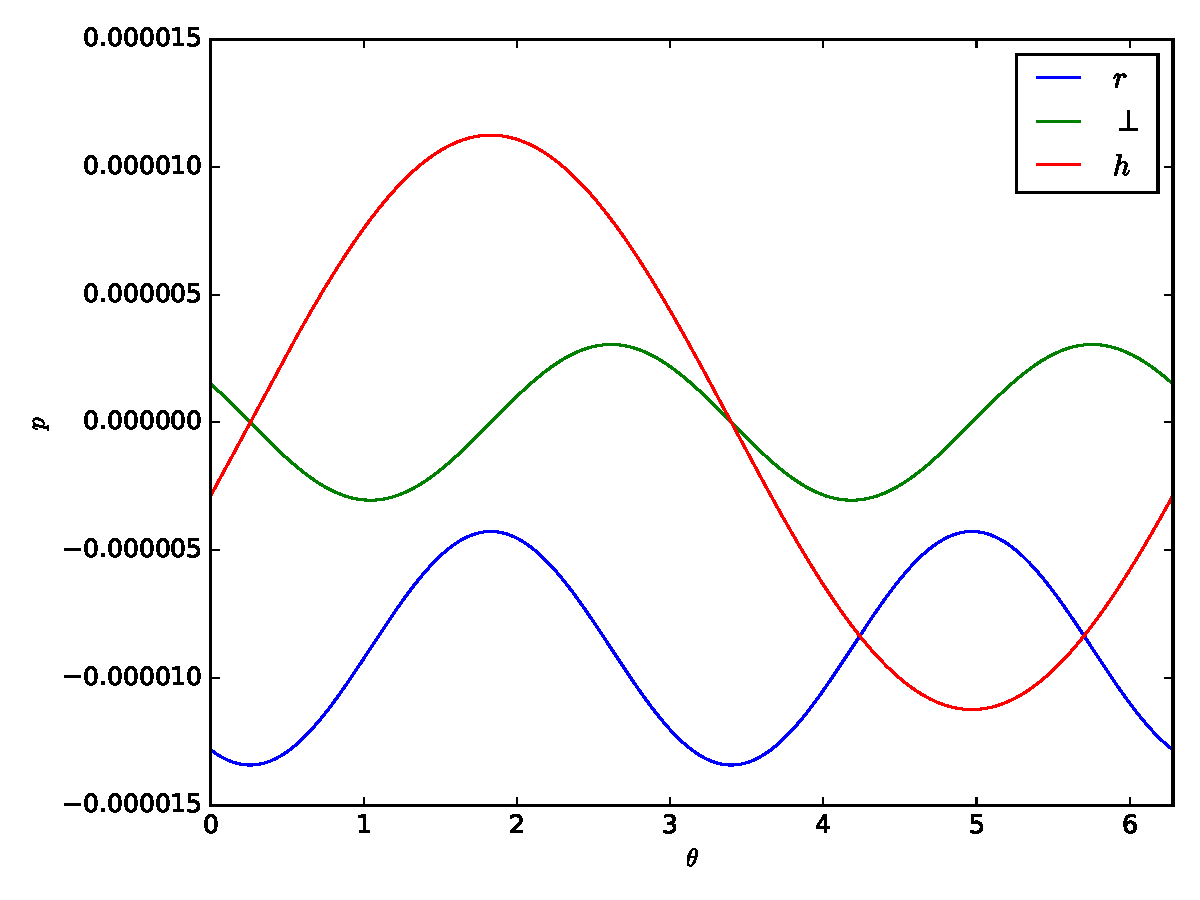
\includegraphics[height=0.55\textheight]{p4.pdf}
% \label{fig:on}
\end{center}
\caption{Magnitude of perturbing gravitational effects, assuming a constant $R=r=6946$km.}
\end{figure}


\clearpage
\problem{}
\textit{Drag forces:}
\begin{enumerate}
\item Estimate the drag force imposed on the HST at its actual altitude, and also as if it were at ISS altitude. Do this for two cases, solar min and solar max, using the NASA atmospheric model you used in HW \#2. Assume a non-rotating Earth. List all other assumptions.
\begin{table}[h]
\begin{center}
\begin{tabular}{rrr}
\toprule
    & Low & High \\
\midrule
ISS & 6.370e-16 & 5.138e-15 \\
HST & 4.362e-17 & 4.536e-16 \\
\bottomrule
\end{tabular}
\end{center}
\caption{$\rho$, atmospheric density, at ISS (400km) and HST (500km) altitudes during low and high solar activity (g/cm$^{-3}$).}
\end{table}
\begin{align*}
D &= -\dfrac{1}{2} \rho S C_D v^2_r \left( \dfrac{v_r}{|v_r|} \right)
\end{align*}

We must assume several things to fill out this equation:
\begin{enumerate}
\item We guess the `exposed' surface area, as a constant $S \approx 13.2 \mbox{ m} \cdot 4.2 \mbox{ m} = 55.44 \mbox{ m}$
\item We guess a value for the coefficient of drag, $C_D \approx 2.5$
\item We specify an approximate velocity of HST, $v_r = 6.47 \hat{x} + 1.97 \hat{y} - 3.45 \hat{z} \mbox{ km/s}$
\end{enumerate}
Plugging in these values, we arrive at:
\begin{table}[h]
\begin{center}
\begin{tabular}{rrr}
\toprule
    & Low & High \\
\midrule
ISS & 2.54e-09 & 2.05e-08 \\
HST & 1.74e-10 & 1.81e-09 \\
\bottomrule
\end{tabular}
\end{center}
\caption{$D$, atmospheric drag, at ISS (400km) and HST (500km) altitudes during low and high solar activity (Newtons).}
\end{table}

\begin{figure}[tbh!]
\begin{center}
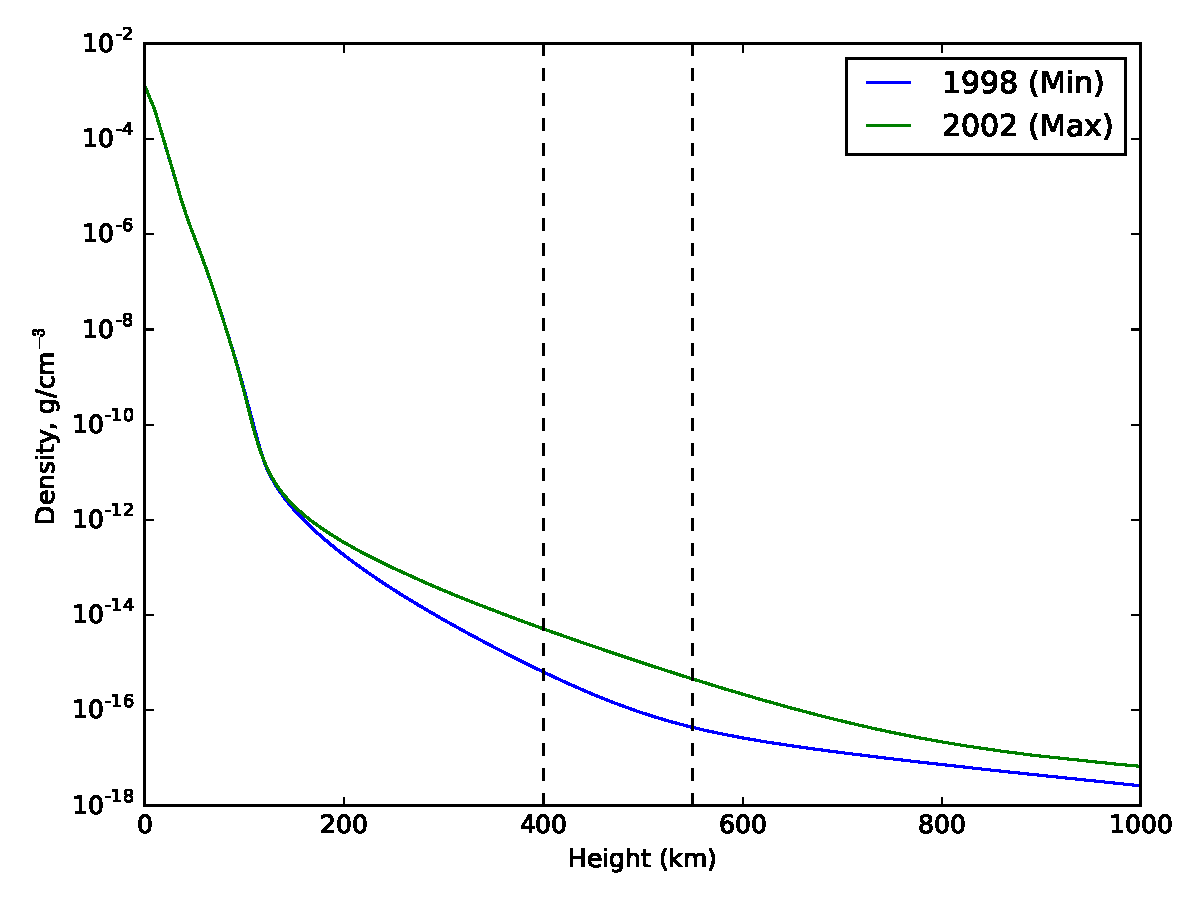
\includegraphics[height=0.4\textheight]{p5.pdf}
% \label{fig:on}
\end{center}
\caption{Atmospheric density by altitude during solar min and solar max.}
\end{figure}

\begin{figure}[tbh!]
\begin{center}
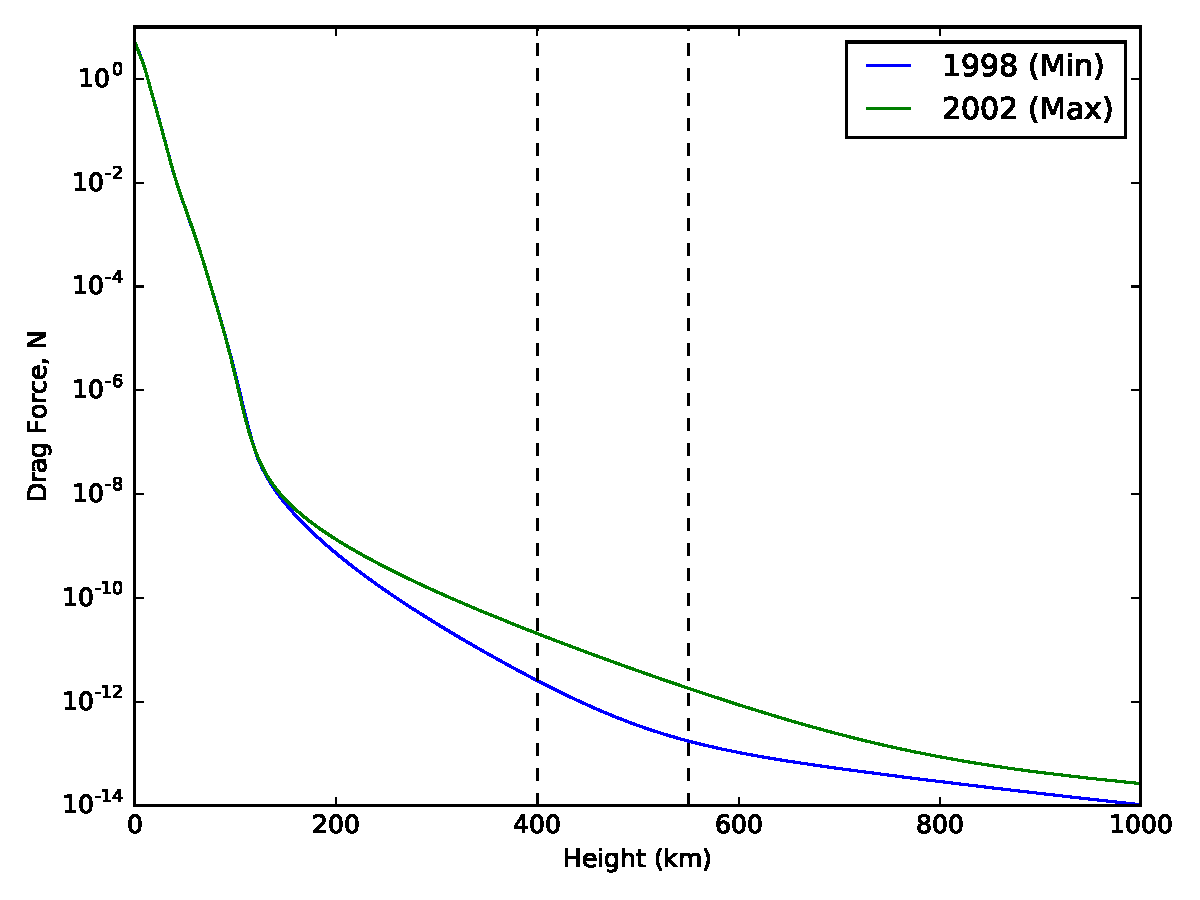
\includegraphics[height=0.4\textheight]{p5b.pdf}
% \label{fig:on}
\end{center}
\caption{Atmospheric drag by altitude during solar min and solar max.}
\end{figure}

\item Explain why drag tends to circularize an elliptical orbit.
\end{enumerate}
Drag is largest at perigee, as this is when both velocity and atmospheric density are the largest. Energy is lost at lower altitudes of elliptical orbits, leaving less velocity to push back out to apogee. Velocity continues to be reduced the most at the lowest part of the orbit until drag is constant throughout the orbit, at which point the orbit is circularized.

\clearpage
\problem{}
\textit{Referring to the Gaussian form of the Lagrange Planetary Equations (eqn 4.34 in the text):}
\begin{enumerate}
\item For a retrograde burn, which orbital parameters will change, and by which sign?
\item To change the orbital inclination, you must burn ``out of plane''. What other orbital parameters will this change, if any?
\item To increase the argument of perigee, in which direction(s) could you generate thrust?
\item For a purely in-plane burn, what is the relationship between tangential and radial thrust required to leave the argument of perigee unchanged?
\end{enumerate}

\clearpage
\problem{}
\textit{Numerical propagation of perturbed orbits:}
\begin{enumerate}
\item Use the HST state vector found in Problem 3 as your initial conditions.
\item Write the orbital equation of motion for perturbed orbits as two first order ODE’s in \textbf{r} and \textbf{v}:
\begin{align*}
\dfrac{d}{dt} \begin{bmatrix}
          \textbf{r} \\
          \textbf{v} \\
        \end{bmatrix}
  = \begin{bmatrix}
          \textbf{v} \\
          \textbf{a} \\
        \end{bmatrix}
  = \begin{bmatrix}
          \textbf{v} \\
          -\mu \dfrac{\textbf{r}}{r^3} + \textbf{p} \\
        \end{bmatrix}
\end{align*}
\item The perturbation vector \textbf{p} is due to drag only, $\textbf{p} = -1/2 \rho v(C_D S)v$.
\item Using RK4, solve for \textbf{r} and \textbf{v} on the time interval of one orbit, once with drag and once without. Plot the
difference over time for the magnitudes of \textbf{r} and \textbf{v}.
\end{enumerate}

\bibliographystyle{IEEEtran}

% \appendix
% \section{Python Code}
% \lstinputlisting{hw3.py}

\end{document}
